\documentclass[12pt]{article}

\usepackage{hyperref}
\usepackage[T1]{fontenc}
\usepackage{float}
\usepackage{enumitem}
\usepackage[french]{babel}
\usepackage{amssymb}
\usepackage{dsfont}
\usepackage{booktabs}
\usepackage{siunitx}
\usepackage{amsmath}
\usepackage{graphicx}
\usepackage{systeme}
\usepackage{caption}
\hypersetup{
    colorlinks=true,
    linkcolor=blue,      % Couleur des liens internes (sections, etc.)
    urlcolor=magenta,    % Couleur des liens vers le Web
    citecolor=green      % Couleur des citations bibliographiques
}
\usepackage{subcaption}
\usepackage{lipsum}
\usepackage{xcolor}
\usepackage{hyperref}
\usepackage[letterpaper,top=2cm,bottom=2cm,left=3cm,right=3cm,marginparwidth=1.75cm]{geometry}
\usepackage{amssymb}
\def\nbR{\ensuremath{\mathrm{I\! R}}}
% Définition d'une couleur bleue pour les liens
\definecolor{bleu}{RGB}{0,0,150}
\hypersetup{
    colorlinks=true,
    allcolors=blue
}
\usepackage{algorithm}
\usepackage{algorithmic}
\usepackage[
backend=biber,
style=authoryear,
]{biblatex}
\usepackage{csquotes}
\addbibresource{references.bib}
\usepackage{tikz}
\usetikzlibrary{shapes,arrows,positioning,calc,decorations.pathreplacing}
\usepackage{enumitem}
\setlist[itemize,1]{label=\textbullet}


% DEBUT DU DOCUMENT 

\begin{document}

% Page titre
\begin{titlepage}
    
    \newcommand{\HRule}{\rule{\linewidth}{0.5mm}}
    \centering

    % EN-TÊTE

    \textsc{\LARGE ENSEIRB-MATMECA}\\[1.5cm]
    \textsc{\large Parcours Mathématiques et Mécanique}\\[0.5cm]

    % TITRE

    \HRule \\[0.4cm]
    { \huge \bfseries Étude et implémentation du raffinement adaptatif de maillage h-adaptatif pour la simulation d'écoulements multiphasiques en une dimension.}\\[0.4cm]
    \HRule \\[1.5cm]

    % AUTEURS ET PROFESSEURS

    \begin{minipage}{0.4\textwidth}
    \begin{flushleft} \large
    \emph{Auteurs :}\\
    \textsc{KNEPFLER Yann }
    \end{flushleft}
    \end{minipage}
    \hfill
    \begin{minipage}{0.4\textwidth}
    \begin{flushright} \large

    \emph{Maître de stage :}\\
    D. .\textsc{de Carvalho}
    \emph{Professeur référent :}\\
    N. \textsc{Barral}
    \end{flushright}
    \end{minipage}\\[2cm]

    % DATE

    {\large 24 septembre 2026}\\[2cm]

    % LOGO

    \includegraphics[width=0.8\textwidth]{Figures/logo_enseirb-matmeca-min.png}

    \vfill

\end{titlepage}

\section*{Résumé}
Dans ce rapport est décrit dans un premier temps l'équation et les méthodes de dsicrétisatiom employés au sein du laboratoire.
Grâce à cela on mesure la pertinence de la méthode de raffinement de maillage adaptatif pour ces problèmes. 
Par la suite, la méthode de maillage adaptatif est introduite et expliquée.
L'explication se fait à travers la structure de maillage utilisée, la façcon d'utiliser ce type de structure et la méthode pour modifier le maillage pour obtenir le raffinement voulu.
Pour avoir une idée plus claire de la manipulation de ces structures, l'implémentation de la méthode est décrite pour expliauer les structures de données utilisées et certains algorithme pour comprendres la place du jeu de paramètre introduit.
Enfin cette méthode est testée sur un cas simple pour mettre en évidence les problèmes rencontrés.


\tableofcontents
\newpage



\section*{Introduction}

Pour pouvoir acheminer efficacement le pétrole du forage sous-marin jusqu'à la plateforme pétrolière if faut pouvoir déterminer de nombreux paramètres clefs de l'écoulement diphasique qu sein du réseau de tuyau, comme la pressioon, la vitesse des phases, ou les fractions volumique. 
Étant donné la taille des réseaux de tuyaux, les schémas numériques implémentés sont des schémas à une dimension. 
Le laboratoire dans leauel j'ai réalisé mon stage cherche à implémenter des méthode de haut ordre de convergence pour obtenir des simulations plus précises.
Cependant les schémas de haut ordre ne sont pas viable si la solution admet des discontinuités, ainsi l'ordre des méthodes est réduit autour des discontinuités.
Il semble alors pertinent de raffiner le maillage autour de ces discontinuités et comme ces dernières se propage au sein de l'écoulement il semble judicieu d'utiliser une méthode de raffinement de maillage daptatif. 

\section{Modèle physique }
\subsection{Description du modèle}
Le modèle utiliser est un modèle à quatre équations d'écoulement diphasique compressible et isotherme en dimension 1. Dans ce modèle on considère que la pression au sein des deux fluides est égale. Ce modèle est une adaptation de celui décrit dans \cite{Wang15}.

\subsection{Formulation mathématiques}

L'équation de continuité du fluide \(k\), où \(k = 1,2\), est
\begin{equation}
    \frac{\partial( \alpha _k \rho _k)}{\partial t}  + \frac{\partial (\alpha _k \rho _k u_k) }{\partial x} = 0
    \label{continuity}
\end{equation}
où \(\alpha_k\) est le fraction volumique du fluide \(k\), \(\rho _k\) est la masse volumique du fluide \(k\) et \(u_k\) la vitesse du fluide \(k\) dans la direction du tuyau.

L'équation de quantité de mouvement du fluide \(k\) est 
\begin{equation}
    \begin{split}
        \frac{\partial (\alpha _k \rho _k u_k)}{\partial t} + \frac{\partial (\alpha _k \rho _k u_k^2)}{\partial x} = - \alpha _k \frac{\partial p _k}{\partial x} - (p_k - p_k^i) \frac{\partial \alpha _k}{\partial x} &+ \\
        \alpha _k \rho _k sin(\theta) + \frac{4 \tau _{k, W}}{D_{H, k}} + \frac{\alpha \tau _i S _i}{A _k}
    \end{split}
    \label{momentum}
\end{equation}
où, \(p_k\) est la pression au sein du fluide \(k\), \(p_k^i\) est la pression a l'interface entre les deux fluides, \(\theta\) la pente du du tuyau, \(\tau _{k, W}\) la contrainte de cisaillement due à la paroi, \(D_{H, k}\) le diamètre hydraulique, \(\tau _i\) la contrainte de cisaillement due à l'interface entre les deux fluides, \(S_i\) le périmètre d'interface et \(A_k\) la surface occupée par le fluide \(k\) dans la section normale.

Pour fermer ce système d'équation on a,
\begin{equation}
    \alpha_1 + \alpha_2 = 1
    \label{closur}
\end{equation}

Pour assurer la stabilité une différence de pression \(\Delta p \) est introduite (\cite{Wang15}).



\section{Méthode numérique}
\subsection{Discrétisation}

La discrétisation se fait sur deux maillages décalés \ref{staggered_grid}, où sur le maillage primaire (en ligne continue) les variables scalaires sont définies et sur un maillage secondaire (en ligne pointillée) les variables vectorielles (vitesse) sont définies. Cette configuration de maillage décrite dans \cite{Patankar80}

\begin{figure}[htbp]
    \centering
    \begin{tikzpicture}[scale=1.1, >=stealth]




% Maillage primaire

% Lignes
\draw[thick] (3, 2) -- (11, 2);
\draw[thick] (3, 0) -- (11, 0);

\draw[thick] (3, 0) -- (3, 2);
\draw[thick] (5, 0) -- (5, 2);
\draw[thick] (7, 0) -- (7, 2);
\draw[thick] (9, 0) -- (9, 2);
\draw[thick] (11, 0) -- (11, 2);


% Nœuds
\filldraw (4, 1) circle  (2.5pt);
\node[above left] at (4, 1) {\(W\)};

\filldraw (6, 1) circle  (2.5pt);
\node[above left] at (6, 1) {\(P\)};

\filldraw (8, 1) circle  (2.5pt);
\node[above left] at (8, 1) {\(E\)};

\filldraw (10, 1) circle  (2.5pt);
\node[above left] at (10, 1) {\(F\)};

% Bords
\node[below] at (5, -0.15) {\small \(w\)};
\node[below] at (7, -0.15) {\small \(e\)};
\node[below] at (9, -0.15) {\small \(ee\)};

% Variables
\node[below] at (4, -0.4) {\small \( ( \alpha, \rho, p)_{W} \) };
\node[below] at (6, -0.4) {\small \( ( \alpha, \rho, p)_{P} \) };
\node[below] at (8, -0.4) {\small \( ( \alpha, \rho, p)_{E} \) };
\node[below] at (10, -0.4) {\small \( ( \alpha, \rho, p)_{F} \) };

% Maillage dual

% Lignes
\draw[dashed, red, very thick] (3, 2) -- (11, 2);
\draw[dashed, red, very thick] (3, 0) -- (11, 0);

\draw[dashed, red, very thick] (4, 0) -- (4, 2);
\draw[dashed, red, very thick] (6, 0) -- (6, 2);
\draw[dashed, red, very thick] (8, 0) -- (8, 2);
\draw[dashed, red, very thick] (10, 0) -- (10, 2);

% Nœuds
\draw[dotted, red, very thick] (3, 1) circle (2.5pt);

\draw[dotted, red, very thick] (5, 1) circle (2.5pt);
\node[below right] at (5, 1) {\(W^S\)};

\draw[dotted, red, very thick] (7, 1) circle (2.5pt);
\node[below right] at (7, 1) {\(P^S\)};

\draw[dotted, red, very thick] (9, 1) circle (2.5pt);
\node[below right] at (9, 1) {\(E^S\)};

\draw[dotted, red, very thick] (11, 1) circle (2.5pt);
\node[below right] at (11, 1) {\(F^S\)};

% Bords
\node[below] at (6, 0) {\small \(w^S\)};
\node[below] at (8, 0) {\small \(e^S\)};

% Variables
\node[above] at (5, 2) {\small \(u_W^S\)};
\node[above] at (7, 2) {\small \(u_P^S\)};
\node[above] at (9, 2) {\small \(u_E^S\)};

% Flux 
\draw[->, very thin] (2.7, 1) -- (3.3, 1);
\draw[->, very thin] (4.7, 1) -- (5.3, 1);
\draw[->, very thin] (6.7, 1) -- (7.3, 1);
\draw[->, very thin] (8.7, 1) -- (9.3, 1);
\draw[->, very thin] (10.7, 1) -- (11.3, 1);



\end{tikzpicture}
    \caption{maillages décalés (adapté de \cite{Ruiz12})}
    \label{staggered_grid}
\end{figure}

Cette configuration de maillage permet de prévenir les phénomènes de découpages pair/impair qui interviennent qu sien des algorithmes de corrections de la pression (\cite{Patankar80}).

Avant la discrétisation des équations, les terme advectifs des équations de quantité de mouvement de chaque phase (\ref{momentum}) sont linéarisés pour faciliter la résolution numérique (\cite{Wang15}), et l'on soustrait l'équation de continuité multiplié par \(u_k\) pour les deux phases:
\begin{equation}
    (\alpha_k \rho_k) \frac{\partial u_k}{\partial t} + ( \alpha_k \rho_k u_k) \frac{\partial u_k}{\partial x} = - \alpha_k \frac{\partial p_k}{\partial x} - \Delta p \frac{\partial \alpha_k}{\partial x} + \alpha_k \rho_k g sin\theta + \frac{4 \tau_{k, W}}{ D_{H, k} } + \frac{\alpha_k \tau_i S_i}{A_k}
    \label{befor_discretization}
\end{equation}

Après avoir discrétisé l'équation \ref{befor_discretization} sur le maillage secondaire on obtient à l'aide de la méthode des volumes finis on obtient le terme à gauche suivant:
\begin{equation}
    LHS = (\alpha_k \rho_k)_e^n \frac{u_{k,e}^{n+1} - u_{k, e}^{n} }{\Delta t} + (\alpha_k \rho_k u_k)_e^n \left( \frac{u_k}{\Delta x} \right)_e^n
    \label{LHS}
\end{equation}

Dans le laboratoire plusieurs méthodes numériques sont implémenté, deux méthode classique, schéma upwind du premier ordre et le schéma monotone décentré en amont (schéma MUSCL), et un schéma de reconstruction de flux. Les variables scalaires \(\alpha_k\) et \(\rho_k\) sont évaluées sur le maillage secondaire par interpolation.

Le second membre de l'équation (\ref{befor_discretization}) est discrétisé de la façon suivante, 
\begin{equation}
    \begin{split}
        RHS = - \alpha_{k, e}^n \frac{p_E^{n+1} - p_P^{n+1}}{\Delta x} - \Delta p _{k, e}^n \frac{\alpha_{k, E}^n - \alpha_{k, P}^n}{\Delta x} &+ \\
        (\alpha_k \rho_k)_e^ngsin\theta + \left( \frac{4 \tau_{k, W}}{D_{H, k}} \right)_e^n + \left( \frac{\alpha_k \tau_i S_i}{A_k} \right)_e^n
    \end{split}
    \label{RHS}
\end{equation}

Les équations de continuités sont discrétisées sur le maillage primaire:
\begin{equation}
    \frac{(\alpha_k \rho_k)_P^{n+1} - (\alpha_k \rho_k)_P^n}{\Delta t} + \left( \frac{\alpha_k \rho_k u_k}{\Delta x } \right)_P^n = 0
\end{equation}

\subsection{Exemple de cas test}
\label{section: Exemple_cas_test}
Les schémas implémentés sont testés sur le problème classique du robinet (\cite{Harten83}): dans un tuyau vertical, rempli d'eau et d'air, de l'eau est injecté par le dessus du tuyau. L'écoulement de l'eau est ensuite accélérer à cause de la gravité et d'un gradient de pression et de l'air rentre par le bas du tuyau.
La figure (\ref{cas_test}) montre que pour ce cas test il y a une discontinuité se propageant en fonction du temps. Étant donné aue le théorème de la barrière de Godunov assure aue seule un schéma d'ordre 1 peut conserver la monotonie si la solution admet des discontinuités, les schémas implémentés varient localement en ordre autour de ces discontinuité.
C'est pourquoi il serait pertinent de raffiner le maillage autour de ces mêmes zones autour des dicontinuité pour augmenter la précsion des schémas.

\begin{figure}[htbp]
    \centering 
    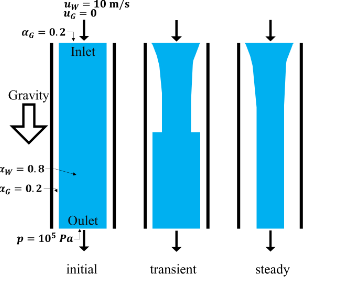
\includegraphics[width=0.6\textwidth]{figures/cas_test.png}
    \caption{Schéma du problème du robinet (adapté de \cite{Ruiz12})}
    \label{cas_test}
\end{figure}

\section{Méthode de raffinement de maillage adaptatif}

La méthode de maillage adaptatif consiste à estimer les zones produisant le plus d'erreur, autour de forts gradients ou de discontinuités, et de raffiner le maillage autour de ces zones.
En général, la méthode ne dépend pas du système d'équations à résoudre ni du schéma.
\subsection{Configuration du maillage }
\subsubsection{Structure de maillages imbriqués}
\label{section: structure de maillage imbriqués}

Pour le raffinement de maillage adaptatif on utilise une suite de maillage uniformes imbriqués (\cite{Berger_Collela98}). On note les niveaux de raffinements \( l = 1, ..., l_{max} \), où le niveau \(1\) est le plus grossier, et on définit, 
\begin{equation}
    G_l = \bigcup_k G_{l, k}.
\end{equation}

On a alors un unique maillage au niveau \( l = 1 \) et ce maillage recouvre entièrement le domaine. Pour chaque niveau de maillage on définit \( h_l \) la largeur des mailles au sein des maillages au niveau \( l \). On définit également un ratio de raffinement de la façon suivante \( r = \frac{h_{l-1}}{h_l} \), ce ratio est un entier et ici on choisit \( r = 2 \).

\begin{figure}[htbp]
    \centering
    \begin{tikzpicture}[scale=1.1, >=stealth]

    % Maillage principal

    % ligne horizontale
    \draw[thick] (2, 6) -- (10, 6);

    % lignes verticales
    \draw[thick] (2, 5.5) -- (2 , 6.5);
    \draw[thick] (3, 5.75) -- (3 , 6.25);
    \draw[thick] (4, 5.75) -- (4 , 6.25);
    \draw[thick] (5, 5.75) -- (5 , 6.25);
    \draw[thick] (6, 5.75) -- (6 , 6.25);
    \draw[thick] (7, 5.75) -- (7 , 6.25);
    \draw[thick] (8, 5.75) -- (8 , 6.25);
    \draw[thick] (9, 5.75) -- (9 , 6.25);
    \draw[thick] (10, 5.5) -- (10 , 6.5);

    % Anotations
    \node[right] at (10, 6) {  \( G_{1,1} \)};

    % Maillages au niveau 2

    % lignes horizontales
    \draw[thick] (3, 4) -- (6, 4);
    \draw[thick] (8, 4) -- (10, 4);

    % lignes vertical
    \draw[thick] (3, 3.5) -- (3, 4.5);
    \draw[thick] (6, 3.5) -- (6, 4.5);
    \draw[thick] (8, 3.5) -- (8, 4.5);
    \draw[thick] (10, 3.5) -- (10, 4.5);
    \draw[thick] (3.5, 3.75) -- (3.5, 4.25);
    \draw[thick] (4, 3.75) -- (4, 4.25);
    \draw[thick] (4.5, 3.75) -- (4.5, 4.25);
    \draw[thick] (5, 3.75) -- (5, 4.25);
    \draw[thick] (5.5, 3.75) -- (5.5, 4.25);
    \draw[thick] (8.5, 3.75) -- (8.5, 4.25);
    \draw[thick] (9, 3.75) -- (9, 4.25);
    \draw[thick] (9.5, 3.75) -- (9.5, 4.25);

    % Anotations
    \node[right] at (6, 4) {\( G_{2,1} \) };
    \node[right] at (10, 4) {\( G_{2,2} \) };


    % Maillage au niveau 3

    % ligne horizontale
    \draw[thick] (3.5, 2) -- (4.5, 2);

    % lignes verticales 
    \draw[thick] (3.5, 1.5) -- (3.5, 2.5);
    \draw[thick] (4.5, 1.5) -- (4.5, 2.5);
    \draw[thick] (4.25, 1.75) -- (4.25, 2.25);
    \draw[thick] (3.75, 1.75) -- (3.75, 2.25);
    \draw[thick] (4, 1.75) -- (4, 2.25);
    
    % Anotations 
    \node[right] at (4.5, 2) {\( G_{3,1}\)};

    % Échelle
    \draw[->, thick] (0, 6) -- (0, 1);
    \draw[thick] (-0.25, 6) -- (0.25, 6);
    \draw[thick] (-0.25, 4) -- (0.25, 4);
    \draw[thick] (-0.25, 2) -- (0.25, 2);

    \node[above right] at (0, 1) {\( l \)};
    \node[above right] at (0, 6) {\( 1 \)};
    \node[above right] at (0, 4) {\( 2 \)};
    \node[above right] at (0, 2) {\( 3 \)};

    % Liaisons entre les maillages
    \draw[dashed, thick, gray] (3, 4.5) -- (3, 5.75);
    \draw[dashed, thick, gray] (6, 4.5) -- (6, 5.75);
    \draw[dashed, thick, gray] (8, 4.5) -- (8, 5.75);
    \draw[dashed, thick, gray] (10, 4.5) -- (10, 5.5);
    \draw[dashed, thick, gray] (3.5, 2.5) -- (3.5, 3.75);
    \draw[dashed, thick, gray] (4.5, 2.5) -- (4.5, 3.75);
    



    
\end{tikzpicture}
    \caption{Structure de maillages imbriqués}
    \label{nested_grid}
\end{figure}

Pour assurer la bonne imbrication des maillages entre eux il faut que, 
\begin{itemize}
    \item Un maillage au niveau \(l\) doit commencer et se finir au coin d'une maille du même maillage au niveau \(l-1\).
    \item Un maillage au niveau \(l-1\) doit séparer un maillage au niveau \(l\) et un maillage au niveau \(l-2\)
    \item Une maille au niveau \(l\) peut uniquement avoir des mailles voisines au niveau \(l, \; l-1, \; \text{ou} \; l+1\)
\end{itemize}

On définit maillage mère de \( G_{l, k} \) comme le maillage au niveau \(l-1\) dans lequel \( G_{l, k} \) est "contenu", et on dit que \( G_{l, k} \) est un maillage fille de \( G_{l-1, q} \) si \( G_{l-1, q} \) est le maillage mère de \( G_{l, k} \). 

\subsubsection{Définition des conditions de bords}
Pour pouvoir avancer un maillage d'un pas de temps il faut lui assigner des condition de bord. Pour cela on définit des mailles fantômes aux bords des maillages, décrite dans \cite{Berger_Collela98}. Le choix du nombre de mailles fantômes sur chaque côté du maillage dépend du schéma utilisé.
Sur la figure \ref{ghost_cells} on met en evidence les mailles fantômes (en pointillé) d'un maillage raffiné \( G_{l, k} \) pour un problème où le domaine de définition est \( [0, 1] \). 
En notant \(U_{(m, q), i}^n\) le vecteur solution dans la maille \( i\) du maillage \(G_{m, q}\) à l'iteration n, et en prenant la figure \ref{ghost_cells} comme exemple, on définit les mailles fantômes de la façon suivante; 

\begin{itemize}
    \item À l'interface avec le maillage parent, \( U_{(l, k), -1}^n = U_{(l, k), 0}^n = U_{(l-1, q), I}^n \) 
    \item À l'interface avec la bordure du domaine les valeurs de \( U_{(l, k), n+1} \; \text{et} \;  U_{(l, k), n+2}\) sont définies à l'aide des conditions de bord. 
\end{itemize}

\begin{figure}[htbp]
    \centering
    \begin{tikzpicture}

    % axe des abscisses
    \draw[->, thick] (-1, 3.5) -- (10,3.5);
    \draw[thick] (0, 3.25) -- (0, 3.75);
    \draw[thick] (8, 3.25) -- (8, 3.75);

    \node[below right] at (10, 3.5) {\( x \)};
    \node[below right] at (0, 3.5) {\( 0 \)};
    \node[below right] at (8, 3.5) {\( 1 \)};

    
    % maillage parent
    
    % ligne horizontale
    \draw[thick] (0, 2) -- (8, 2);

    % lignes verticales
    \draw[thick] (0, 1.5) -- (0, 2.5);
    \draw[thick] (8, 1.5) -- (8, 2.5);
    \draw[thick] (2, 1.75) -- (2, 2.25);
    \draw[thick] (4, 1.75) -- (4, 2.25);
    \draw[thick] (6, 1.75) -- (6, 2.25);

    % Annotations
    \node[right] at (-1.5, 2) {\(G_{l-1, p}\)};
    \node[above] at (3, 2) {\(I\)};

    % maillage secondaire

    % ligne horizontale    
    \draw[thick] (4, 0) -- (8, 0);

    % lignes verticales
    \draw[thick] (4, -0.5) -- (4, 0.5);
    \draw[thick] (8, -0.5) -- (8, 0.5);
    \draw[thick] (5, -0.25) -- (5, 0.25);
    \draw[thick] (6, -0.25) -- (6, 0.25);
    \draw[thick] (7, -0.25) -- (7, 0.25);

    % Mailles fantômes
    \draw[dashed, thick] (2, 0) -- (4, 0);
    \draw[dashed, thick] (8, 0) -- (10, 0);
    \draw[dashed, thick] (2, -0.25) -- (2, 0.25);
    \draw[dashed, thick] (3, -0.25) -- (3, 0.25);
    \draw[dashed, thick] (9, -0.25) -- (9, 0.25);
    \draw[dashed, thick] (10, -0.25) -- (10, 0.25);

    % Annotations
    \node[right] at (-1.5, 0) {\(G_{l, k}\)};
    \node[above] at (2.5, 0.4) {\small \(-1\)};
    \node[above] at (3.5, 0.4) {\small \(0\)};
    \node[above] at (4.5, 0.4) {\small \(1\)};
    \node[above] at (7.5, 0.4) {\small \(n\)};
    \node[above] at (9.5, 0.4) {\small \(n+1\)};
    \node[above] at (8.5, 0.4) {\small \(n+2\)};
    



    


\end{tikzpicture}
    \caption{Maillage avec mailles fantômes pour 2 mailles fantômes de chaque côté}
    \label{ghost_cells}
\end{figure}

\subsubsection{Corretions des maillages grossiers}
Après avoir intégré l'équation sur les maillages filles d'un maillage \( G_{l, k}\) les zones raffinées du maillage mère sont corriger en utilisant les valeurs calculés sur les maillages filles et pour assurer la conservation, on applique une correction de flux aux mailles autour des zones raffinées (\cite{Berger_Leveque98}).

\begin{figure}[htbp]
    \centering
    \begin{tikzpicture}
    
   % maillage parent
    
    % ligne horizontale
    \draw[thick] (-0.1, 2) -- (8.1, 2);

    % lignes verticales
    \draw[thick] (0, 1.75) -- (0, 2.25);
    \draw[thick] (8, 1.75) -- (8, 2.25);
    \draw[thick] (2, 1.75) -- (2, 2.25);
    \draw[thick] (4, 1.75) -- (4, 2.25);
    \draw[thick] (6, 1.75) -- (6, 2.25);

    % Annotations
    \node[right] at (-1.5, 2) {\small \(G_{l-1, p}\)};
    \node[above] at (3, 2) {\small \(I\)};

    % maillage secondaire

    % ligne horizontale    
    \draw[thick] (2, 0) -- (6, 0);

    % lignes verticales
    \draw[thick] (2, -0.5) -- (2, 0.5);
    \draw[thick] (6, -0.5) -- (6, 0.5);
    \draw[thick] (3, -0.25) -- (3, 0.25);
    \draw[thick] (4, -0.25) -- (4, 0.25);
    \draw[thick] (5, -0.25) -- (5, 0.25);

    % Annotations
    \node[right] at (-1.5, 0) {\small \( G_{l, k} \)};
    \node[below] at (2.5, 0) {\small \(1\)};
    \node[below] at (3.5, 0) {\small \(2\)};
    \node[below] at (4.5, 0) {\small \(3\)};
    \node[below] at (5.5, 0) {\small \(4\)};

    % liaisons entre maillage
    \draw[dashed, thick, gray] (2, 0.5) -- (2, 1.75);
    \draw[dashed, thick, gray] (6, 0.5) -- (6, 1.75);

    % Correction des mailles raffinées
    \draw[->, thick, green] (2.5, 0.2) -- (2.9, 1.8);
    \draw[->, thick, green] (3.5, 0.2) -- (3.1, 1.8);
    \draw[->, thick, green] (4.5, 0.2) -- (4.9, 1.8);
    \draw[->, thick, green] (5.5, 0.2) -- (5.1, 1.8);

    % Correction des flux
    \draw[->, thick, blue] (2.4, 1) -- (1.6, 1);
    \draw[->, thick, blue] (5.6, 1) -- (6.4, 1);
\end{tikzpicture}
    \caption{Correction des mailles raffinées}
    \label{correction_overlapping}
\end{figure}

En prenant en l'example de la figure \ref{correction_overlapping}, on corrige les mailles raffinées (flèches vertes) de la façon suivante; 
\[ 
U_{(l-1, p), I}^{n+1} = \frac{1}{2}(U_{(l, k), 1}^{n+1} + U_{(l, k), 2}^{n+1} ) 
\] 
On note les flux d'une maille \(m\) vers une maille \(m+1\) sur un maillage \(G_{l, k}\) calculer à partir de la solution à l'iteration n \( F_{i+1}^n \).
On corrige alors le flux pour les mailles autour de la zone raffinée (flèches en bleu) de la façon suivante,
\[
U_{(l-1, p), I-1 }^{n+1} := U_{(l-1, p), I-1 }^{n+1} - \frac{k}{h_{l-1}} \left( F_{(l, k), 1}^n - F_{(l-1, p), I}^n \right)
\]
\[
U_{(l-1, p), I + 2}^{n+1} := U_{(l-1, p), I + 2}^{n+1} + \frac{k}{h_{l-1}} \left( F_{(l, k), 5}^n - F_{(l-1, p), I+2}^n \right)
\]


\subsection{Raffinement de Maillage}
Pour raffiner une suite de mailles accollées d'un maillage \(G_{l, k}\) on crée un maillage fille \(G_{l+1, p}\) de cette suite de mailles.
Pour initialiser le nouveau maillage fille, on prolonge les valeurs du maillage mère de sorte que \[\frac{1}{h_l} \int_{\text{maille mère}} U dV = \frac{1}{h_{l+1}}\sum_{\text{mailles filles}} \int_{\text{maille fille}} UdV\] (\cite{Berger_Oliger84}). Donc en prenant la figure \ref{grid_prolongation} comme exemple, on prolonge de la façon suivante, 
\begin{align*}
    U_{(l+1, p), 0}^n = U_{(l, k), I}^n - \frac{1}{4} \text{slope}_I^n\\
    U_{(l+1, p), 1}^n = U_{(l, k), I}^n + \frac{1}{4} \text{slope}_I^n
\end{align*}

Où \(\text{slope}_I^n \) est le limiteur de pente, ici le limiteur minmod, telle que, 
\[
    slope_I^n = 
    \begin{cases}
        0, \text{si } (\Delta U_{(l, k), I}^n) (\Delta U_{(l, k), I+1}) \leq 0 \\
        \text{sgn}(\Delta U_{(l, k), I}^n) \; \text{min}(|\Delta U_{(l, k), I}^n|, \; |\Delta U_{(l, k), I+1}|), \text{sinon}
    \end{cases}
\]
et \(\Delta U_{(l, k), I}^n = U_{(l, k), I}^n - U_{(l, k), I-1}^n\).


\begin{figure}[htbp]
    \centering
    \begin{tikzpicture}
        
    % lignes horizontales
    \draw[thick] (-0.1, 2) -- (8.1, 2);
    \draw[thick] (2, 0) -- (6, 0);

    % lignes verticales
    \draw[thick] (0, 1.75) -- (0, 2.25);
    \draw[thick] (8, 1.75) -- (8, 2.25);
    \draw[thick] (2, -0.5) -- (2, 0.5);
    \draw[thick] (6, -0.5) -- (6, 0.5);
    \draw[thick] (2, 1.75) -- (2, 2.25);
    \draw[thick] (4, 1.75) -- (4, 2.25);
    \draw[thick] (6, 1.75) -- (6, 2.25);
    \draw[thick] (3, -0.25) -- (3, 0.25);
    \draw[thick] (4, -0.25) -- (4, 0.25);
    \draw[thick] (5, -0.25) -- (5, 0.25);

    % liaisons entre les maillages 
    \draw[dashed, thick, gray] (2, 0.5) -- (2, 1.75);
    \draw[dashed, thick, gray] (6, 0.5) -- (6, 1.75);

    % prolongqtion du maillage fille 
    \draw[->, thick, green] (2.9, 1.8) -- (2.5, 0.2);
    \draw[->, thick, green] (3.1, 1.8) -- (3.5, 0.2);
    \draw[->, thick, green] (4.9, 1.8) -- (4.5, 0.2);
    \draw[->, thick, green] (5.1, 1.8) -- (5.5, 0.2);

    % Annotations
    \node[left] at (-0.1, 2) {\(G_{l, k}\)};
    \node[left] at (-0.1, 0) {\(G_{l+1, p}\)};

    \node[above] at (3, 2.1) {\(I\)};
    \node[above] at (5, 2.1) {\(I+1\)};

    \node[below] at (2.5, -0.1) {\(1\)};
    \node[below] at (3.5, -0.1) {\(2\)};
    \node[below] at (4.5, -0.1) {\(3\)};
    \node[below] at (5.5, -0.1) {\(4\)};

\end{tikzpicture}
    \caption{Prolongation d'un maillage fille}
    \label{grid_prolongation}
\end{figure}

\subsection{Estimateur d'erreur}
Pour déterminer les zones à raffiner on utilise un estimateur d'erreur.
Ici on utilise un estimateur d'erreur a posteriori, qui estime l'erreur commise après avoir intégré le problème sur le maillage.
Ici l'estimateur d'erreur utilisé est l'estimateur de Löhner (\cite{Löhner86}) permettant de localiser les discontinuités, 
\[
    E_i = \frac{|U_{i+1} - 2 U_i + U{i-1}|}{|U_{i+1} - U_i| + |U_i - U_{i-1}| + \epsilon (|U_{i+1}| + 2|U_i| + |U_{i-1}|)}
\]
où \(\epsilon\) est un paramètre dépendant du problème, permettant de filtrer les perturbations. 

\section{Implémentation}
Le but était de créer une librairie facilement adaptable pour différents schémas numériques et différents estimateurs d'erreurs. L'implémentation réalisée esr une adaptation du code Fortran90 \cite{Hawke18} en Julia.

\subsection{Structures de données}  
On définit la structure de maillage qui contient des informations sur la solution, le maillage mère, les maillages filles, la position dans l'espace du maillage et la position au sein du maillage mère du maillage.
On définit également la structure de niveau qui contient une liste de maillage au même niveau de raffinement, ainsi que le niveau mère et le niveau. 
Ainsi les structure sont reliés en arborescence, comme décrit dans la figure \ref{grid_hierarchy}.

\begin{figure}[htbp]
    \centering
    \begin{tikzpicture}

    % lignes horizontales
    \draw[dashed, thick] (0, 0) -- (12, 0);
    \draw[dashed, thick] (0, 3) -- (12, 3);
    \draw[dashed, thick] (0, 6) -- (12, 6);
    \draw[dashed, thick] (0, 9) -- (12, 9);

    % Maillages

    % cercles
    \draw[thick] (9, 7.5) circle (30pt);
    
    \draw[thick] (7.5, 4.5) circle (30pt);
    \draw[thick] (10.5, 4.5) circle (30pt);

    \draw[thick] (7.5, 1.5) circle (30pt);

    % Lien entre les maillages
    
    \draw[<->, thick] (7.5, 5.57) -- (7.9, 7.05);
    \draw[<->, thick] (10.5, 5.57) -- (10.1, 7.05);
    
    \draw[<->, thick] (7.5, 2.56) -- (7.5, 3.44);

    % Annodtations
    \node at (9, 7.5) {\large \(G_{1, 1}\)}; 
    \node at (7.5, 4.5)  {\large \(G_{2, 1}\)}; 
    \node at (10.5, 4.5) {\large \(G_{2, 2}\)}; 
    \node at (7.5, 1.5) {\large \(G_{3, 1}\)}; 


    % Niveaux
    \node at (2, 7.5) {\large \(G_1\)};
    \node at (2, 4.5) {\large \(G_2\)};
    \node at (2, 1.5) {\large \(G_3\)};

    % liaisons entre les niveaux 
    \draw[<->, thick] (2, 4.8) -- (2, 7.2);
    \draw[<->, thick] (2, 1.8) -- (2, 4.2);


\end{tikzpicture}
    \caption{Exemple de structures de données}
    \label{grid_hierarchy}
\end{figure}

\subsection{Algorithmes}

Pour pouvoir intégrer un maillage il faut que ses mailles fantômes soient bien définies, c'est pourquoi l'intégration des niveaux se fait à partir du niveau le plus gros jusqu'au niveau le plus grossier dans l'algorithm \ref{advance_level}.
Étant donné que dans (\ref{RHS}), on remarque que la résolution de la pression est implicite, les mailles fantômes doivent être définies à partir des valeurs à l'itération \(n+1\) pour pouvoir intégrer l'équation à l'itération \(n\) sur le maillage. 
Comme ce même algorithm est récursif un niveau maximum de raffinement est défini pour pouvoir contrôler au mieux le nombre de niveau.

\begin{algorithm}
    \caption{Intégration d'un niveau}
    \label{advance_level}
    \begin{algorithmic}
    \STATE \textbf{Données:} niveau \(G_l\)
    \STATE Intégrer la solution sur les maillages de \(G_l\)
    \IF {\(l < l_{max}\)}
    \STATE Mettre à jour les mailles fantômes des maillages filles des maillages de \(G_l\)
    \STATE Appliquer cette algorithme au niveau \(G_{l+1}\)
    \STATE Corriger les mailles raffiner et les flux au bords des zones raffinées
    \STATE Applique l'algorithme de raffinement au niveau \(G_l\)
    \ENDIF
\end{algorithmic}
\end{algorithm}

Il est préférable de prendre une zone de raffinement plus large que les tolérances préconisent pour faire en sorte que les zones où le plus d'erreur est commis reste dans les zones raffinées une fois intégré l'équation (\cite{Löhner86}).
C'est pourquoi on introduit le paramètre \texttt{buffer\_width} dans l'algorithme \ref{refine_level}.
Dans ce même algorithme deux tolérances sont introduites puisque une tolérance plus faible pour les mailles déjà raffinée est utile pour des schémas présentants de la diffusion numérique.
En effet, la diffusion numérique lisse les solutions et ainsi plus l'équation est intégré plus l'estimation d'erreur calculée est faible.

\begin{algorithm}
    \caption{Raffinement d'un niveau}
    \label{refine_level}
    \begin{algorithmic}
    \STATE \textbf{Data:} niveau \(G_l\), largeur de la zone tampon \texttt{buffer\_width}, tolérance de raffinement \texttt{ref\_tol}, tolérance de grossissement \texttt{coars\_tol} 
    \STATE Appliquer l'estimateur d'erreur à l'ensemble des mailles de \(G_l\)
    \STATE Maquer les mailles pour le raffinement à une distance de \texttt{buffer\_width} des mailles dont l'estimation d'erreur dépasse \texttt{ref\_tol} et des mailles précédement raffinées dont l'estimation d'erreur dépasse \texttt{coars\_tol}.
    \STATE Créer et prolonger de nouveaux maillages filles la où les mailles ont été marqués pour le raffinement
    \STATE Copier les valeurs des anciens maillages filles sur les nouveaux
    \STATE Associer les maillages du niveau \(G_{l+1}\) aux maillages \(G_{l+2}\)
\end{algorithmic}
\end{algorithm}

Pour empêcher la destruction d'un maillage fille qui possède lui même des maillages filles, dans l'algorithme \ref{compute_error} on force le raffinement dans ce cas en donnant une estimation d'erreur virtuel haute.
Grâce à cela et les zones de raffinement plus large, la bonne imbriquation défini dans la section \ref{section: structure de maillage imbriqués} est assurée.

\begin{algorithm}
    \caption{Estimateur d'erreur}
    \label{compute_error}
    \begin{algorithmic}
    \STATE \textbf{DATA:} maille \(\Omega\)
    \STATE Appliquer la formule de l'estimateur de Löhner
    \STATE Si \(\Omega\) est raffinées au moins deux fois, mettre l'estimation d'erreur à 1
\end{algorithmic}
\end{algorithm}

\section{Application}
\subsection{Configuration}
\label{section: configuration}
La méthode implémentée est testée sur l'équation d'advection en 1 dimension pour plusieurs conditions initiales,

\begin{equation}
    \begin{cases}
            \frac{\partial u}{\partial t} + \frac{\partial u}{\partial x} = 0, \quad \text{où } x \in [0, 1] \\
            u(0, x) = u_0(x) \\
            u(t, 0) = u_0(-t)\\
            u(t, 1) = u_0(1-t)
    \end{cases}
\end{equation}

Les conditons initiales sont, 
\begin{itemize}
    \item La gaussienne, \(u_0(x) = 0.9exp(-(\frac{x - x_c}{\sigma})^2) + 0.1\) où \(x_c  = 0.25\) et \(\sigma = 0.05\)
    \item Le créneau, \( u_0(x) = \begin{cases} 1, \text{si } x < 0.2 \\ 0, \text{sinon} \end{cases} \)
    \item Le signal rectangle, \( u_0(x) = \begin{cases} 1, \text{si } 0.1 < x < 0.2 \\ 0, \text{sinon} \end{cases} \)
\end{itemize}

L'équation est intégrée grâce au schéma upwind du premier ordre.

\subsection{Validation}
La méthode est testé en mesurant l'ordre de convergence pour un nombre maximum de niveau allant de 1 à 4. 
Le jeu de paramètre pour ce test est le suivant, 
\begin{itemize}
    \item \texttt{ref\_tol}: 0.00009375
    \item \texttt{coars\_tol}: 0.00003125
    \item \texttt{buffer\_width}: 4
    \item \(\epsilon\) : 0.01
    \item coefficient cfl: 0.5
\end{itemize}

L'ordre de convergence est mesuré uniquement sur la première condition initiale, étant donné quelle est la seule continue.
Étant donné que pour les quatres nombres maximum de niveau de raffinement l'ordre de convergence est proche de 1 sur la figure (\ref{convergence}), on peut considérer que la méthode est valide.
Sur cette figure, l'axe des abscisses représente la taille des mailles du maillage le plus grossier.
\begin{figure}[htbp]
    \centering
    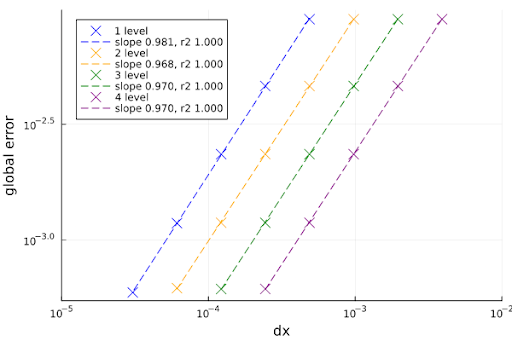
\includegraphics[width=0.8\textwidth]{figures/validation.png}
    \caption{Courbe de convergence}
    \label{convergence}
\end{figure}

\subsection{Analyse}
\label{section: analyse}
La méthode est également testé sur les trois conditions initiales en mesurant l'erreur globale pour différent nombres maximum de niveaux de raffinement, \(l_{max}\).
Ici le nombre de mailles du maillage le plus grossier est fixé à 64, et le jeu de paramètre est (\cite{Löhner86}),

\begin{itemize}
    \item \texttt{ref\_tol}: 0.3
    \item \texttt{coars\_tol}: 0.1
    \item \texttt{buffer\_width}: 4
    \item \(\epsilon\) : 0.01
    \item coefficient cfl: 0.5
\end{itemize} 

Pour respecter la condition cfl sur tout les niveaux, le pas de temps choisi est le pas de temps du niveau le plus fin. Puisque le schéma d'Euler explicite admet une forte diffusion numérique, en augmentant le nombre de niveaux l'effet de la diffusion numérique sur les maillages les plus grossiers est amlifié.
C'est pourquoi il y a peu de différence en terme d'erreur globale lorsqu'on augmente \(l_{max}\) sur le tableau \ref{tableau}.
De plus pour ce jeu de paramètre, l'erreur globale pour \(l_{max} = 3\) et \(l_{max} = 4\) est égale pour la condition initiale de la gausssienne. Ceci est attendu puisque pour \(l_{max} = 4\) il y a seulement 3 niveaux de raffinement.
Ainsi la solution est assez précise avec 3 niveaux de raffinements pour que les tolérance ne soient pas atteintes par l'estimateur d'erreur. Alors l'estimateur d'erreur fonctionne détecte plus facilement les forts gradients des solutions discontinues, ce qui est le but rechercher d'aprés lasection \ref{section: Exemple_cas_test}. 



\begin{table}[htbp]
    \begin{tabular}{|c|c|c|c|}
        \hline
        \(l_{max}\) / condition initiale & Gaussienne & Créneau & Signal rectangle \\
        \hline
        1 & 0,08012983661 & 0,09126679464 & 0,135470096 \\
        2 & 0,06978615294 & 0,07682885266 & 0,110086436 \\
        3 & 0,05254172054 & 0,0708716789 & 0,1009166435 \\
        4 & 0,05254172054 & 0,06958670085 & 0,09985460564 \\
        
        \hline        
    \end{tabular}
    \caption{Erreur globale en fonction de \(l_{max}\) et de la condition initiale}
    \label{tableau}
\end{table}

\section{Conclusion}

Durant ce stage, le modèle physique et les schémas numériques utilisé par le laboratoire ont été étudiés pour pouvoir se rendre compte des enjeux du raffinement de maillage adaptatif liés à ce problème.
Ensuite  la méthode de maillage adaptatif a été étudier, puis testé sur un cas simple.
Pour le moment, on ne peut pas conclure de l'efficacité de la methode de raffinement de maillage adatatif présenté ici appliquer qu probl`me du laboratoir.
Cependant le choix de l'estimateur d'erreur de Löhner semble être correct, étant donné sa capacité à localiser les discontinuité.\\

\textbf{Perspectives d'amélioration}

Pour finaliser l'étude de la méthode implémenter, il faudrait la tester sur un schéma implicite et sur de différents estimateur d'erreur, pour assurer le caractère adaptable.
Pour améliorer la méthode et éviter de trop fortes diffusions numériques, il faudrait que chaque niveau de raffinement ait son propre pas de temps, et respecte la condition cfl à son niveau.










\newpage
\printbibliography
\end{document}